%!TEX TS-program = xelatex
%!TEX encoding = UTF-8 Unicode
\documentclass[a4paper, 12pt, oneside]{book}

\usepackage{cite}
%\usepackage{chapterbib}
%The chapterbib package facilitates multiple bibliographies in a LATEX document
\usepackage[hyphens]{url}
%Verbatim with URL-sensitive line breaks.
\usepackage[colorlinks=true,linkcolor=black,citecolor=black,filecolor=blue,urlcolor=blue,unicode]{hyperref}
%The hyperref package is used to handle cross-referencing commands in LaTeX to produce hypertext links in the document. The package provides backends for the \special set defined for HyperTeX DVI processors; for embedded pdfmark commands for processing by Acrobat Distiller (dvips and Y&Y’s dvipsone); for Y&Y’s dviwindo; for PDF control within pdfTeX and dvipdfm; for TeX4ht; and for VTeX’s pdf and HTML backends.
\usepackage{verbatim}
%The verbatim environment  simply reproduces every character you input, including all  s p a c e s!
\usepackage{color}
%you can set the color of the font of the text, and set the background color of the page.
\usepackage[dvipsnames]{xcolor}
%xecolor package is a simple package which defines about 140 different colors by XeTeX's font
\usepackage{graphicx}
%Standard LaTeX graphics.
\usepackage{array}
%The array environment is used to make a table of information, with column alignment (left, center, or right) and optional vertical lines separating the columns.
\usepackage{gensymb}
%Provides generic commands \degree, \celsius, \perthousand, \micro and \ohm which work both in text and maths mode.
\usepackage{indentfirst}
%Make the first line of all sections etc., be indented by the usual paragraph indentation. This should work with all the standard document classes. This minimalist package is part of the "tools" bundle in the LaTeX required distribution.
\usepackage{algorithm}
\usepackage{algpseudocode}
%A suite of tools for typesetting algorithms in pseudo-code. The algorithmicx package provides many possibilities to customize the layout of algorithms. You can use one of the predefined layouts (pseudocode, pascal and c and others), with or without modifications, or you can define a completely new layout for your specific needs.
\usepackage{enumitem}
%Control layout of itemize, enumerate, description.  It supersedes both enumerate and mdwlist (providing well- structured replacements for all their funtionality), and in addition provides functions to compute the layout of labels, and to 'clone' the standard environments, to create new environments with counters of their own.
\usepackage{mfirstuc}
%\makefirstuc{〈stuff 〉} This makes the first object of 〈stuff 〉 uppercase unless 〈stuff 〉 starts with a con- trol sequence followed by a non-empty group, in which case the first object in the group is converted to uppercase.
\usepackage{fancyvrb}
%This package provides very sophisticated facilities for reading and writing ver- batim TEX code.
\usepackage{amsfonts}
%TeX fonts from the American Mathematical Society.
\usepackage{ifmtarg}
%If-then-else command for processing potentially empty arguments.
\usepackage{amsmath}
%The amsmath package is a LATEX package that provides miscellaneous enhance- ments for improving the information structure and printed output of documents that contain mathematical formulas.
\usepackage{amssymb}
% Math symbols
\usepackage[mathcal]{euscript}
%This file sets up some font shape definitions to use the Euler script symbols in math mode.
\usepackage[notbib]{tocbibind}
%Add (or disable) bibliography/index/contents to Table of Contents.
\usepackage{rotating}
%Rotation tools, including rotated full-page floats.
\usepackage{hhline}
%The command \hhline produces a line like \hline, or a double line like \hline\hline, except for its interaction with vertical lines. The command takes a preamble (rather like the preamble of a tabular environment), and this specifies whether there are to be one or two horizontal lines, and what happens when the horizontal line meets a vertical one. The package is part of the tools bundle in the LaTeX required distribution.
\usepackage{wallpaper}
%Easy addition of wallpapers (background images) to LaTeX documents, including tiling.
\usepackage{pdfpages}
%Include PDF documents in LaTeX.
\usepackage{pst-fractal,pst-exa}
% The package will draw the Julia and Mandelbrot sets, the Sierpinski triangle, Koch flake, and Apollonius Circle as well as fractal trees (which need not be balanced) with a variety of different parameters (including varying numbers of iterations).

\usepackage{afterpage} % ntut
% http://tex.stackexchange.com/questions/36880/insert-a-blank-page-after-current-page


%Define \XeTeX \XeLaTeX command
\def\reflect#1{{\setbox0=\hbox{#1}\rlap{\kern0.5\wd0
 \special{x:gsave}\special{x:scale -1 1}}\box0 \special{x:grestore}}}
\def\XeLaTeX{\leavevmode
 \setbox0=\hbox{X\lower.5ex\hbox{\kern-.15em\reflect{E}}\kern-.08em\LaTeX}%
 \dp0=0pt\ht0=0pt\box0}
 \def\XeTeX{\leavevmode
 \setbox0=\hbox{X\lower.5ex\hbox{\kern-.15em\reflect{E}}\kern-.08em\TeX}%
 \dp0=0pt\ht0=0pt\box0}

% \usepackage[none]{hyphenat}  %hyphenation package

% Start Declare physics symbols
\newcommand{\gv}[1]{\ensuremath{\mbox{\boldmath$ #1 $}}}
\newcommand{\grad}[1]{\gv{\nabla} #1} % for gradient
\let\divsymb=\div % rename builtin command \div to \divsymb
\renewcommand{\div}[1]{\gv{\nabla} \cdot #1} % for divergence
\newcommand{\curl}[1]{\gv{\nabla} \times #1} % for curl
\let\baraccent=\= % rename builtin command \= to \baraccent
\renewcommand{\=}[1]{\stackrel{#1}{=}} % for putting numbers above =
%end Declare

\usepackage{tabularx}
%tabularx, is defined, which takes the same arguments as tabular*, but modifies the widths of certain columns, rather than the inter column space, to set a table with the requested total width. The columns that may stretch are marked with the new token X in the preamble argument. This package requires the array package. The package is part of the tools bundle in the LaTeX required distribution.
\usepackage{lmodern}
%The Latin Modern family of fonts consists of 72 text fonts and 20 mathematics fonts, and is based on the Computer Modern fonts released into public domain by AMS (copyright © 1997 AMS).
\font\lmr="[lmroman10-regular]"

\usepackage{listings}
%Typeset source code listings using LaTeX.
\usepackage{textcomp}
%provide many text symbols (such as baht, bullet, copyright, musicalnote, onequarter, section, and yen)

\usepackage{amsthm}
%The package facilitates the kind of theorem setup typically needed in American Mathematical Society publications. The package offers the theorem setup of the AMS document classes (amsart, amsbook, etc.) encapsulated in LaTeX package form so that it can be used with other document classes. Amsthm is part of the (required) AMS-LaTeX distribution, so should be present in any LaTeX distribution.
\newtheorem{mydef-no-caption}{Definition}
\newenvironment{mydef}[1][]%
	{\begin{mydef-no-caption}{\ifnotmtarg{#1}{\textnormal{(\textbf{#1})}~}}}%
	{\end{mydef-no-caption}}

\usepackage{numprint}
%Print numbers with separators and exponent if necessary.
\npthousandsep{,}
\npthousandthpartsep{}
\npdecimalsign{.}

\usepackage{multirow}
%Create tabular cells spanning multiple rows.

\usepackage{ntut} %ntut
%NTUT thesis style file
\hypersetup{
	pdfauthor={\authorEN{}},
	pdftitle={\titleEN{}},
	pdfsubject={NTUT Thesis} % ntut
}

\usepackage{setspace}
%Set space between lines.

\usepackage[absolute]{textpos}
%Place boxes at arbitrary positions on the LaTeX page.
\lstdefinestyle{nonumbers}{numbers=none}
\textblockorigin{0mm}{0mm}

\setcounter{tocdepth}{2}

\pagestyle{plain}




% ntut
\usepackage{titlesec}
\usepackage{titletoc}
\usepackage{CJKnumb}
%\titleformat{\chapter}{\centering\Huge\bfseries}{第\,\CJKnumber{\thechapter}\,章}{1em} {}
%\titleformat{\chapter}{\centering\huge\bfseries}{第\,\CJKnumber{\thechapter}\,章}{1em} {}
\titleformat{\chapter}{\centering\LARGE\bfseries}{第\,\CJKnumber{\thechapter}\,章}{1em} {}
%\titleformat{\chapter}{\centering\large\bfseries}{第\,\CJKnumber{\thechapter}\,章}{1em} {}




\begin{document}

%----------- hyphenation  -----------
%\righthyphenmin=10  % Best hyphenation parameter

%----------- watermark -----------
%\CenterWallPaper{0.174}{fig/logo.png}
\CenterWallPaper{0.25}{fig/logo_bg.png}
%\setlength{\wpXoffset}{6.1725cm}  % 控制出現在頁面的位置
%\setlength{\wpYoffset}{10.5225cm} % 控制出現在頁面的位置

%----------- side page, used for printing on spline -----------
\makeside

%----------- cover page -----------
\maketitle

\frontmatter
%----------- generate the certification page by LaTeX -----------
%\makecertification
%----------- includepdf by using package pdfpages -----------
\addcontentsline{toc}{chapter}{口試委員會審定書}
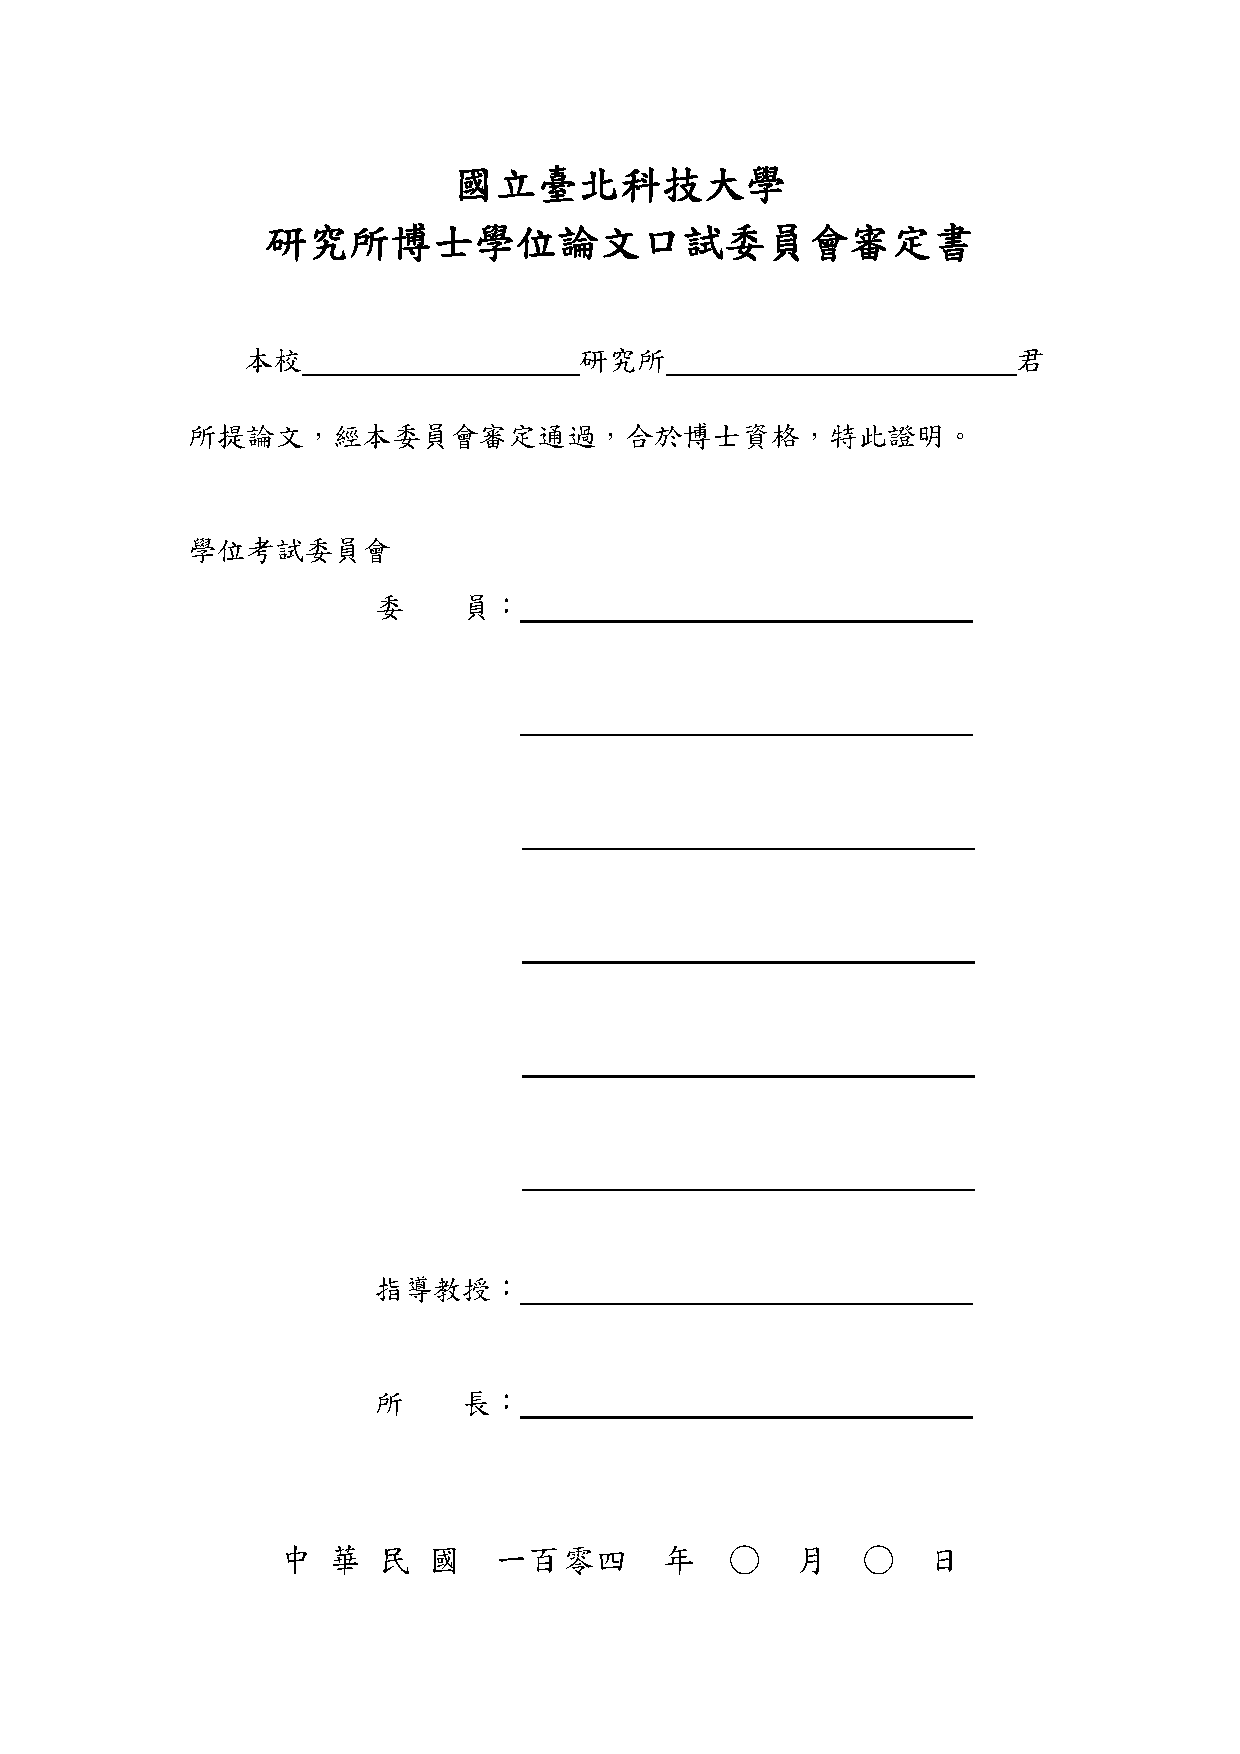
\includepdf{pdf/bb(18).pdf} % 轉檔案成 pdf
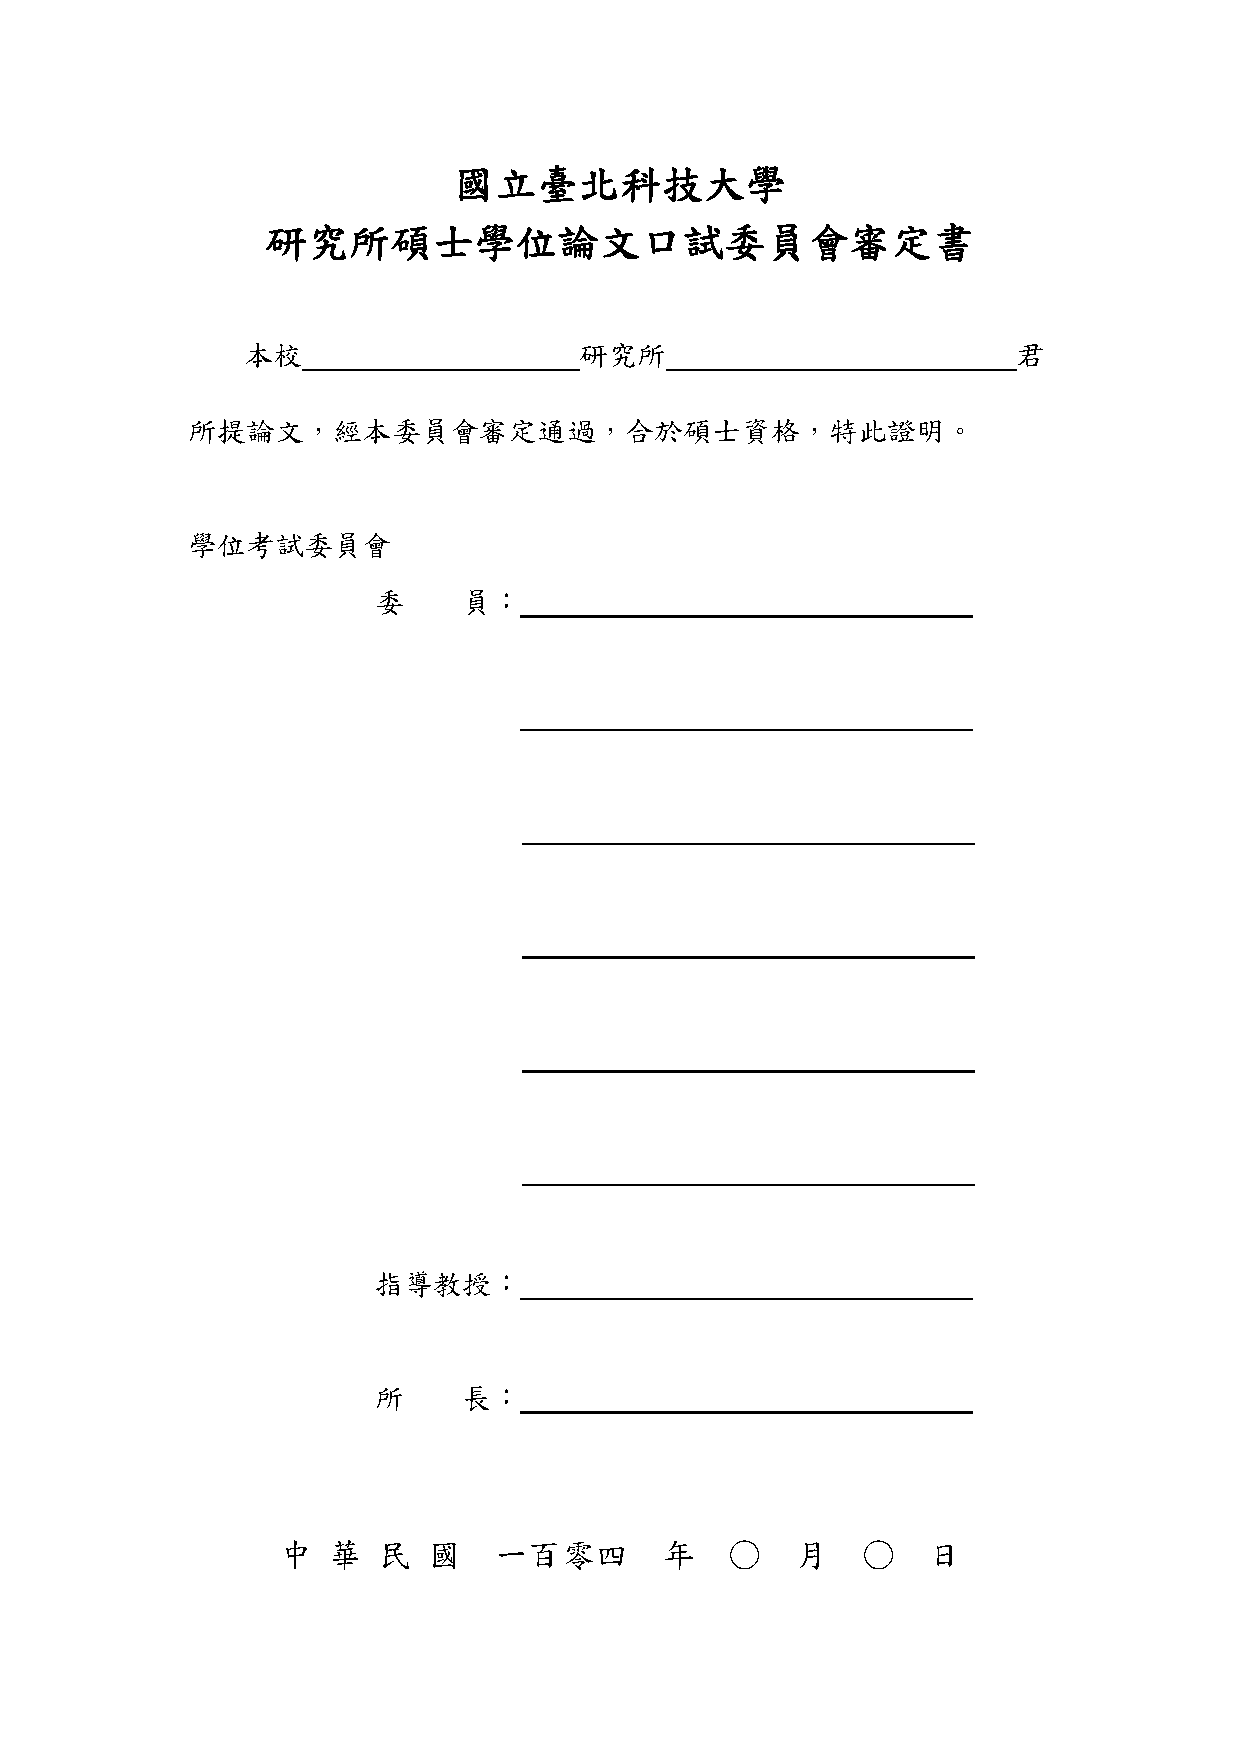
\includepdf{pdf/bb(19).pdf} % 轉檔案成 pdf

%\singlespacing
%\onehalfspacing
\doublespacing
\begin{abstractCH}

\noindent
論文名稱:解析卷積神經網路於物件偵測\\
頁數:五十頁\\
校所別:國立臺北科技大學 資訊工程  研究所\\
畢業時間:一百零七學年度 第二學期\\
學位:碩士\\
研究生:謝柏鋒\\
指導教授:謝東儒 博士\\

\noindent
關鍵詞:YOLO、物件偵測、機器學習\\

近年來,卷積神經網路有許多令人突破性的發展。我們的目的是在於解析最近對於物件偵測技術的性能分類非常良好的YOLO(You Only Look Once)。對於解析深度學習已經有許多相關的論文,但對於解析卷積神經網路的相關論文卻較少,本論文是用簡易的方式說明卷積神經網路的運作方式,並且將過程呈現,可以讓一般大眾更加認識機器學習的運作方式,同時也讓專家方便於解析卷積神經網路的架構,並且能夠迅速改善原本的架構,使其加速。

\end{abstractCH}

\begin{abstractEN}

\noindent
Title: DAnalysis convolutional neural network of object detection\\
Pages: 50\\
School: National Taipei University of Technology\\
Department: Electrical Engineering\\
Time: June, 2019\\
Degree: Master\\
Researcher: PO-FONG HSIEH\\
Advisor: TUNG-JU HSIEH, Ph.D.\\

\noindent
Keywords: \\


Start writing abstract from here. Start writing abstract from here. Start writing abstract from here. Start writing abstract from here. Start writing abstract from here. Start writing abstract from here. Start writing abstract from here. Start writing abstract from here.


\end{abstractEN}

\begin{acknowledgementsCH}

所有對於研究提供協助之人或機構,作者都可在誌謝中表達感謝之意。標題使用20pt粗標楷體,並於上、下方各空一行(1.5倍行高,字型12pt空行)後鍵入內容。致謝頁須編頁碼(小寫羅馬數字表示頁碼)。\\\\



\begin{enumerate}[leftmargin=0pt, topsep=0pt, itemsep=0pt, label=\Roman{*}.]

\item 此範本參考下列網站的資料:
\begin{enumerate}[topsep=0pt, itemsep=0pt, label=$\bullet$]
    \item \href{https://code.google.com/p/ntu-thesis-latex-template/}{台大碩博士論文LaTeX範本}
    \item \href{http://exciton.eo.yzu.edu.tw/~lab/latex/latex_note.html}{陳念波老師的元智大學論文樣板}
    \item \href{https://code.google.com/p/ntust-thesis/}{台灣科技大學同學編寫的碩博士論文Latex模板}
\end{enumerate}

\item 原作者參考並修改自下列網站的資料:
\begin{enumerate}[topsep=0pt, itemsep=0pt, label=$\bullet$]
    \item \href{http://www.csie.ntu.edu.tw/~tzhuan/www/resources/ntu/}{如何用 LaTeX 排版臺灣大學碩士論文}\\
    \textemdash 台灣大學論文\LaTeX\ 樣版原創者\href{http://www.csie.ntu.edu.tw/~tzhuan/www/}{黃子桓}的教學網頁
    \item \href{http://www.hitripod.com/blog/2012/05/latex-thesis-template-quick-reference/}{LaTeX 常用語法及論文範本}\\
    \textemdash \href{http://www.hitripod.com/blog/}{Hitripod}所修改的範本,這裡參考了許多他所寫的格式和內容
    \item \href{http://www.cc.ntu.edu.tw/chinese/epaper/0014/20100920_1404.htm}{使用LaTeX做出精美的論文}
    \item \href{http://www.hitripod.com/blog/2011/04/xetex-chinese-font-cjk-latex/}{XeTeX:解決 LaTeX 惱人的中文字型問題}
    \item \href{http://code.google.com/p/ntuthesis/}{台灣大學碩士、博士論文的Latex模板}\\   
\end{enumerate}

\end{enumerate}


%----------- Have a fractal fern? -----------
%\begin{pspicture}
%\psFern[scale=30,maxIter=100000,linecolor=Green]
%\end{pspicture}

\end{acknowledgementsCH} 

\singlespacing
\tableofcontents

\onehalfspacing
\listoffigures
\listoftables

\mainmatter

\doublespacing

%----------- Include/Input your thesis here -----------
%normal cite == \input

\chapter{導論}
\label{c:1}

%==========================================================================================
\section{導論}
%首先界定您的研究問題的研究領域並說明此領域在廣度上的重要性。
卷積神經網路為近年來在物件偵測及辨識度上表現最為突出的深度學習架構,本論文中,我們選定現在在物件偵測上效能與辨識度最高的YOLO(You Only Look Once)作為解析的範本,介紹卷積神經網路的運作過程,比較其他種物件偵測的演算法,拆解YOLO內部的運作過程,探討YOLO能夠領先於其他演算法的關鍵原因。\\
%指出問題的研究動機:也就是在此研究領域上,有何新研究問題需要被解決? 前人的成果中有那些缺失處或未考慮的因素?或有那一些傳統難題未被徹底解決的?
在卷積神經網路中,目前我們所知若是將神經網路的深度加高,可以提升準確率,但過多的深度卻會造成其效率降低。所以現今大部分的演算法只能使用試誤法,以低效率的方式去測驗比較此演算法,粗略估計此演算法的深度與效能達到平衡,常常會有過高的深度或準確率未達預期的情形發生,為了解決此問題,本論文著重於解析卷積神經網路的架構及其運作方法,以簡單明瞭的方式闡述其過程,並且分析原本架構的問題,改善原本的架構。\\
%與其他的比較
以往的論文幾乎沒有以視覺化的方式解析卷積神經網路的運作原理,所以在本論文中,希望能以簡單清晰的方式讓人們了解卷積神經網路,並且能在網頁上呈現,其操作性較為直覺性,能夠馬上知道目前選取的位置的功能與效果。

%前述的問題期望如何被解決:如降低演算法的時間複雜度或減少電源的耗費或降低網路部署的成本等。儘可能提出明確的方向,如可量化的數量或質性的改善。說明你要解決或是想更進一步瞭解的問題?
%==========================================================================================
\section{Figure}
\label{ss:Figure}
\begin{figure}[htpb!]
  \centering
    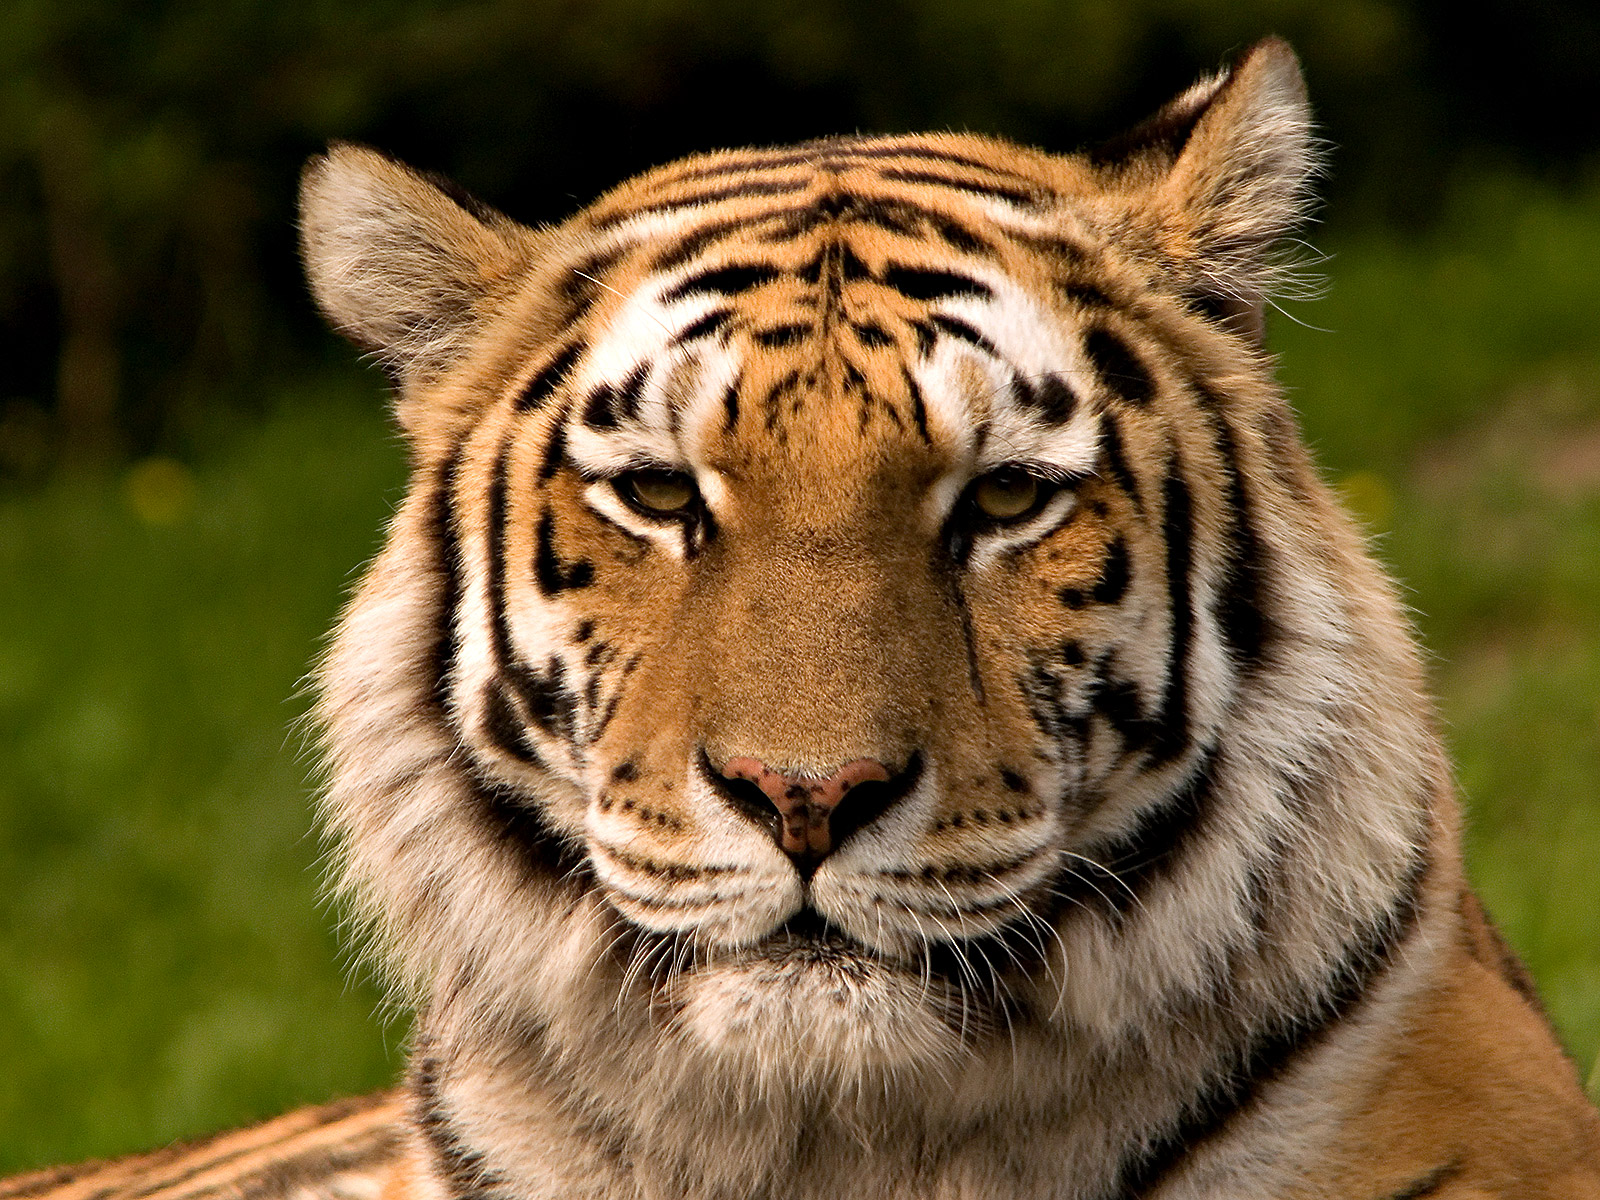
\includegraphics[width=0.5\textwidth]{fig/tiger.jpeg}
    \caption{\label{fig:tiger}A picture of a tiger.}
\end{figure}

Figure~\ref{fig:tiger} is a picture of a tiger.



%==========================================================================================
\section{Table}
\label{ss:Table}

\href{http://en.wikibooks.org/wiki/LaTeX/Tables}{Table examples on WIKIBOOKS}.

\begin{table}[htpb]\begin{center}
\caption{Table Example 1}
\begin{tabularx}{8cm}{llX}
\hline
Start & End  & Character Block Name \\
\hline
3400  & 4DB5 & CJK Unified Ideographs Extension A \\
4E00  & 9FFF & CJK Unified Ideographs \\
\hline
\end{tabularx}
 \end{center}\end{table}

\begin{table}[htpb]\begin{center}
\caption{Table Example 2}
\begin{tabular}{llr}
\hline
\multicolumn{2}{c}{Item} \\
\cline{1-2}
Animal & Description & Price (\$) \\
\hline
Gnat  & per gram & 13.65 \\
      & each     &  0.01 \\
Gnu   & stuffed  & 92.50 \\
Emu   & stuffed  & 33.33 \\
Armadillo & frozen & 8.99 \\
\hline
\end{tabular}
 \end{center}\end{table}

 \begin{table}[htpb]\begin{center}
	\label{t:prefix-table}
	\caption{Table Example 3}
	\renewcommand{\arraystretch}{1.0}
	\begin{tabularx}{300pt}{|c|X| }
		\hline
		\multirow{1}{*}{\textbf{Allocation}} &
		Allocation, Element, Type, Script
		\\ \hline\hline
		%------------------------------
		\multirow{6}{*}{\textbf{Data Types}} &
        Byte2, Byte3, and Byte4\\ &
        Float2, Float3, Float4\\ &
        Int2, Int3, Int4\\ &
        Long2, Long3, Long4\\ &
        Matrix2f, Matrix3f, Matrix4f\\ &
        Short2, Short3, Short4
        \\ \hline\hline
		%------------------------------
		\multirow{4}{*}{\textbf{Graphics}} &
		Mesh\\&
		ProgramFragment, ProgramRaster\\&
		ProgramStore, ProgramVertex\\&
		RSSurfaceView
		\\ \hline
		%------------------------------
	\end{tabularx}
\end{center}\end{table}

\chapter{相關文獻討論}
\label{c:2}
%==========================================================================================
視覺化演算法在CNN上已經有許多相關的研究,一開始的研究著重於將圖片的特徵,但隨著CNN的快速發展,視覺化已經擴展到解釋CNN的整體架構與運作方式。主要是解析每個演算法的網路架構和演算法的邏輯,其中有幾個較具代表性的方法:\\
Erhan 等人提出 Activation Maximization 來對傳統的淺層網路進行解釋。\\
後來,Simonyan 等人通過將單個 CNN 神經元的最大啟用視覺化合成一個輸入影像模式( input image pattern ),進一步改進了這種方法。\\
後續出現了很多工作都是基於這種方法,再利用不同的正則項進行擴充套件,以提高合成影像模式的可解釋性。\\
Mahendran 等人提出了 Network Inversion 重建基於多個神經元啟用的輸入影像,以此說明每個 CNN 層學習到的綜合特徵圖,揭示了 CNN 網路在網路層層面的內部特徵。\\
Network Inversion 根據特定層的特徵圖中的原始影像重建輸入影像,這可以揭示該圖層所儲存的影像資訊。\\
沒有選擇對輸入影像進行重建以實現特徵視覺化,Zeiler 等人提出了基於反摺積神經網路的視覺化方法(Deconvolutional Neural Network based Visualization, DeconvNet),該方法利用 DeconvNet 框架將特徵圖直接對映到影像維度,利用反摺積 CNN 結構(由反摺積層和反摺積層組成)在特定神經元啟用的原始輸入影像中查詢影像模式。
\\通過直接對映, DeconvNet 可以突出顯示輸入影像中的哪些模式啟用特定神經元,從而直接連結神經元和輸入資料的含義。\\
周博磊等人提出了 Network Dissection based Visualization,它從語義層面對 CNN 進行了解釋。\\
通過引用異構影像資料集——Borden,Network Dissection 可以有效地將輸入影像分割為多個具有各種語義定義的部分,可以匹配六種語義概念(例如場景,目標,部件,材質,紋理和顏色)。\\
由於語義直接代表了特徵的含義,神經元的可解釋性可以顯著提高。\\
以上都是圍繞在以CNN為基礎的視覺化,而鮮少有對其他較進階的CNN演算法進行視覺化分析。
%==========================================================================================

%\section{Manga Vectorization and Manipulation with Procedural Simple Screentone.}
%資料來源:\cite{7399427}\par
%影片:\href{video.mp4}{影片}

%==========================================================================================

%\section{YOLO9000:Better, Faster, Stronger.}
%資料來源:\cite{RedmonF17}\par
%影片:\href{YOLO 9000 Better Faster Stronger.mp4}{影片}

%==========================================================================================
%\section{Deep Residual Learning for Image Recognition. 卷積影像深度學習}
%資料來源:{Microsoft Research.2016 IEEE\cite{DBLP:journals/corr/HeZRS15}}
%影片:\href{Research Talk (in Hindi) Deep Residual Learning for Image Recognition.mp4}{影片}

%==========================================================================================

%\section{Only Look Once, Mining Distinctive Landmarks from ConvNet for Visual Place Recognition.只看一次,在ConvNet找到特殊的地標,用於地點識別}
%資料來源:{2017 IEEE/RSJ International Conference on Intelligent Robots and Systems (IROS)\cite{Chen:etal:IROS2017}}\\
%影片:\href{1331_VI.mp4}{影片}

%==========================================================================================

%\section{Visualizing and Understanding Convolutional Networks}
%資料來源:{Dept. of Computer Science,New York University, USA\cite{DBLP:journals/corr/ZeilerF13}}\\
%影片:\href{1331_VI.mp4}{影片}

%==========================================================================================

%\section{Visualizing Convolutional Neural Networks for Image Classification}
%資料來源:{Dept. of Computer Science,New York University, USA\cite{DBLP:journals/corr/abs-1804-11191}}\\
%影片:\href{1331_VI.mp4}{影片}

%==========================================================================================

%\section{Visualization of Neural Network Predictions for Weather Forecasting}
%資料來源:{COMPUTER GRAPHICS forumVolume 00 (2018), number 0 pp. 1–12 \cite{Roesch2017VisualizationON}}\\
%影片:\href{Visualization of Neural Network Predictions for Weather Forecasting (VMV 2017).mp4}{影片}

%==========================================================================================

%\section{Deep learning for computational biology}
%資料來源:{COMPUTER GRAPHICS forumVolume 00 (2018), number 0 pp. 1–12 \cite{Roesch2017VisualizationON}}\\
%影片:\href{Visualization of Neural Network Predictions for Weather Forecasting (VMV 2017).mp4}{影片}

CNN、R-CNN、Fast R-CNN、Faster R-CNN、Mask R-CNN、SSD、YOLO、YOLOv2、YOLOv3……等,都是屬於使用CNN模型,只要輸入一張圖片,並得到該圖片分類的結果,但每個類型所使用的架構並不相同。


\chapter{方法}
\label{c:3}

%==========================================================================================
\section{第一階層子標題}

各階層子標題均應置於左側,並於其下方不空行。

%==========================================================================================
\subsection{第二階層子標題}

第二階層子標題之內文。

%==========================================================================================
\subsubsection{第三階層子標題}

第三階層子標題之內文。


%\bibliographystyle{unsrt}
%\bibliography{thesisbib} 
\chapter{結果與討論}
\label{c:4}

%==========================================================================================
\section{第一階層子標題}

各階層子標題均應置於左側,並於其下方不空行。

%==========================================================================================
\subsection{第二階層子標題}

第二階層子標題之內文。

%==========================================================================================
\subsubsection{第三階層子標題}

第三階層子標題之內文。


\chapter{結論}
\label{c:5}

%==========================================================================================
\section{結論}

各階層子標題均應置於左側,並於其下方不空行。

%==========================================================================================
\section{未來展望}

第二階層子標題之內文。


%\bibliographystyle{unsrt}
%\bibliography{thesisbib} 



%chapter cite  == \include

%\include{start}
%\include{introduction}
%\include{THM}
%\include{EXP}


%\appendix
%----------- Input your appendix here  -----------
%
% this file is encoded in utf-8
% v1.7
%%% 每一個附錄 (附錄一、附錄二、...) 都要複製此段附錄編排碼做為起頭
%%% 附錄編排碼 begin >>>
\newpage
\chapter*{附錄A:第一個附錄名稱} % 修改附錄編號與你的附錄名
\addcontentsline{toc}{chapter}{附錄A:第一個附錄名稱} %建議此內容應與上行相同
\renewcommand{\thechapter}{A} % 如果是附錄二,則內容應為{二}

\setcounter{equation}{0}
\setcounter{figure}{0}
\setcounter{footnote}{0}
\setcounter{section}{0}
\setcounter{subsection}{0}
\setcounter{subsubsection}{0}
\setcounter{table}{0}
%%% <<< 附錄編排碼 end



附錄內容
%
% this file is encoded in utf-8
% v1.7
%%% 每一個附錄 (附錄一、附錄二、...) 都要複製此段附錄編排碼做為起頭
%%% 附錄編排碼 begin >>>
\newpage
\chapter*{附錄B:第二個附錄名稱} % 修改附錄編號與你的附錄名
\addcontentsline{toc}{chapter}{附錄B:第二個附錄名稱} %建議此內容應與上行相同
\renewcommand{\thechapter}{B} % 如果是附錄二,則內容應為{二}

\setcounter{equation}{0}
\setcounter{figure}{0}
\setcounter{footnote}{0}
\setcounter{section}{0}
\setcounter{subsection}{0}
\setcounter{subsubsection}{0}
\setcounter{table}{0}
%%% <<< 附錄編排碼 end



附錄內容
%or %chapter cite  == \include
%%
% this file is encoded in utf-8
% v1.7
%%% 每一個附錄 (附錄一、附錄二、...) 都要複製此段附錄編排碼做為起頭
%%% 附錄編排碼 begin >>>
\newpage
\chapter*{附錄A:第一個附錄名稱} % 修改附錄編號與你的附錄名
\addcontentsline{toc}{chapter}{附錄A:第一個附錄名稱} %建議此內容應與上行相同
\renewcommand{\thechapter}{A} % 如果是附錄二,則內容應為{二}

\setcounter{equation}{0}
\setcounter{figure}{0}
\setcounter{footnote}{0}
\setcounter{section}{0}
\setcounter{subsection}{0}
\setcounter{subsubsection}{0}
\setcounter{table}{0}
%%% <<< 附錄編排碼 end



附錄內容
%%
% this file is encoded in utf-8
% v1.7
%%% 每一個附錄 (附錄一、附錄二、...) 都要複製此段附錄編排碼做為起頭
%%% 附錄編排碼 begin >>>
\newpage
\chapter*{附錄B:第二個附錄名稱} % 修改附錄編號與你的附錄名
\addcontentsline{toc}{chapter}{附錄B:第二個附錄名稱} %建議此內容應與上行相同
\renewcommand{\thechapter}{B} % 如果是附錄二,則內容應為{二}

\setcounter{equation}{0}
\setcounter{figure}{0}
\setcounter{footnote}{0}
\setcounter{section}{0}
\setcounter{subsection}{0}
\setcounter{subsubsection}{0}
\setcounter{table}{0}
%%% <<< 附錄編排碼 end



附錄內容

%
% this file is encoded in utf-8
% v1.7
%%% 每一個附錄 (附錄一、附錄二、...) 都要複製此段附錄編排碼做為起頭
%%% 附錄編排碼 begin >>>
\newpage
\chapter*{符號彙編}
\addcontentsline{toc}{chapter}{符號彙編}
\renewcommand{\thechapter}{符號彙編}

\setcounter{equation}{0}
\setcounter{figure}{0}
\setcounter{footnote}{0}
\setcounter{section}{0}
\setcounter{subsection}{0}
\setcounter{subsubsection}{0}
\setcounter{table}{0}
%%% <<< 附錄編排碼 end

\noindent
Symbol      Meaning\\
Θ			Debye's constant or characteristic temperature\\
Ω			efficiency; number of molecules\\
Ψ			availability of a closed system\\
Δ			internal energy (change) of reaction\\
Φ			availability of a closed system\\
ι			specific irreversibility\\
λ			critical state\\
μ			Joule-Thomson coefficient\\
ν			stoichiometric coefficient (number of moles in chemical equation)\\
ξ			cutoff ratio


\backmatter


%---------- Input your reference here ---------
\renewcommand\bibname{Reference}
\bibliographystyle{unsrt}
\addcontentsline{toc}{chapter}{\bibname}
\bibliography{thesisbib}

%----------- Input your Figure chapter here  -----------
%\input{EndFigTab}
%chapter cite  == \include
%\include{EndFigTab}

\end{document}
